
%(BEGIN_QUESTION)
% Copyright 2006, Tony R. Kuphaldt, released under the Creative Commons Attribution License (v 1.0)
% This means you may do almost anything with this work of mine, so long as you give me proper credit

Determine the voltmeter's indication in this thermocouple circuit (type E) for the following temperatures:

$$\includegraphics[width=15.5cm]{i00381x01.eps}$$

\begin{itemize}
\item{} $T_{measurement}$ = 1500$^{o}$ F ; $T_{reference}$ = 65$^{o}$ F ; Voltmeter voltage = ??? 
\item{} $T_{measurement}$ = 212$^{o}$ F ; $T_{reference}$ = 74$^{o}$ F ; Voltmeter voltage = ??? 
\item{} $T_{measurement}$ = $-$360$^{o}$ F ; $T_{reference}$ = 32$^{o}$ F ; Voltmeter voltage = ??? 
\item{} $T_{measurement}$ = $-$132$^{o}$ F ; $T_{reference}$ = $-$30$^{o}$ F ; Voltmeter voltage = ??? 
\end{itemize}

\underbar{file i00381}
%(END_QUESTION)





%(BEGIN_ANSWER)

\begin{itemize}
\item{} $T_{measurement}$ = 1500$^{o}$ F ; $T_{reference}$ = 65$^{o}$ F ; Voltmeter voltage = 61.145 mV 
\item{} $T_{measurement}$ = 212$^{o}$ F ; $T_{reference}$ = 74$^{o}$ F ; Voltmeter voltage = 4.925 mV 
\item{} $T_{measurement}$ = $-$360$^{o}$ F ; $T_{reference}$ = 32$^{o}$ F ; Voltmeter voltage = $-$9.229 mV 
\item{} $T_{measurement}$ = $-$132$^{o}$ F ; $T_{reference}$ = $-$30$^{o}$ F ; Voltmeter voltage = $-$2.876 mV 
\end{itemize}

%(END_ANSWER)





%(BEGIN_NOTES)


%INDEX% Measurement, temperature: thermocouple

%(END_NOTES)


